\chapter{Experimente}
\label{ch:experimente}

Die verwendeten Metriken der Experimente fassen sich aus Präzision (precision), Erinnerung (recall), F1-Wert (F1-Score) und Genauigkeit (accuracy) zusammen. Zum Berechnen dieser wird das Aufkommen der Richtig Positiven (TP), Falsch Positiven (FP), Falsch Negativen (FN) und Richtig Negativen (TN) Vorhersagen (predictions) des Modells benutzt. Die Kategorie TP zeigt vom Modell richtig erkannte Objekte, welche tatsächlich vorhanden sind, FP bestimmt die falsche Erkennung des Modells von Objekten, die in Wirklichkeit nicht vorhanden sind, FN gibt Auskunft über Objekte, die in der Realität vorhanden sind, das Modell sie allerdings nicht erkannt hat, und TN beschreibt Objekte, die korrekt als nicht vorhanden erkannt wurden.

\[Precision = \frac{TP}{TP + FP}\]

Precision misst den Anteil der korrekten positiven Vorhersagen an allen positiven Vorhersagen des Modells. Sie zeigt, wie genau das Modell bei der Erkennung von Objekten ist und wie gut es falsche positive Ergebnisse vermeidet. Ein hoher Precision-Wert bedeutet, dass wenn das Modell ein Objekt erkennt, es mit hoher Wahrscheinlichkeit tatsächlich vorhanden ist.

\[Recall = \frac{TP}{TP + FN}\]

Recall misst den Anteil der korrekt erkannten positiven Instanzen an allen tatsächlichen positiven Instanzen. Es zeigt, wie gut das Modell alle vorhandenen Objekte einer Klasse findet. Ein hoher Recall-Wert bedeutet, dass das Modell die meisten der tatsächlich vorhandenen Objekte erkennt.

\[F1 = 2 \cdot \frac{Precision \cdot Recall}{Precision + Recall}\]

Der F1-Wert ist das harmonische Mittel aus Precision und Recall. Ein hoher F1-Wert deutet darauf hin, dass das Modell sowohl präzise als auch umfassend in seinen Vorhersagen ist. Der F1-Wert ist besonders nützlich, wenn ein ausgewogenes Verhältnis zwischen Precision und Recall wichtig ist.

\[Accuracy = \frac{TP + TN}{TP + TN + FP + FN}\]

Die Richtigkeit (Accuracy) misst den Anteil aller korrekten Vorhersagen an der Gesamtzahl der Vorhersagen. Sie gibt nur an, wie oft das Modell insgesamt richtig liegt, weshalb sie nur bei der Klassifizierung verwendet wurde.
\\
Zum Visualisieren der Konfusionsmatrizen in diesem Kapitel wurde eine Kombination von \cite{2020SciPy-NMeth, DamianoP2024confusionMatrixGenerator} verwendet.

\section{Objekterkennung}

Für das Unterkapitel der Objekterkennung wurde die Effizienz, verschiedene Diagrammarten aus Texten mithilfe der Ultralytics YOLO Objekterkennungsmodelle zu extrahieren, untersucht. Hierfür wurden die erstellten Datensätze aus \ref{ch:chartbank} zum Vortrainieren und aus \ref{ch:scanbank} zum Feintrainieren verwendet.
\\
Ultralytics YOLO generiert nach abgeschlossenem Modelltraining automatisch verschiedene Metrikseinblicke. Insbesondere das, eines F1-Confidence Diagramms. Aus diesem kann abgelesen werden, wie ein beliebiger Konfidenz Schwellenwert (confidence threshold) der Modellvorhersagen die Evaluationsresultate des F1-Scores beinflusst. Im Folgenden werden für alle Objekterkennungsexperimente jedene Konfidenzwerte gewählt, welche den F1-Wert maximieren.

\subsection{Vortrainiertes Modell auf DocBank}
Um im Verlauf der Datensatzerstellung zu erforschen ob die visuell ähnliche Klassen der Balkendiagramme und Histogramme weiterhin differenziert werden sollen, wurde nach nach dem Erreichen einer Datensatzgröße von 200 Bildern der Datensatz mit Histogrammen, sowie derselbe mit reduzierten Klassen evaluiert.

\subsection*{200 Trainingsbilder (mit Histogramme)}

Aufgrund der limitierten Anzahl an verfügbaren Validationsbildern bei einem so kleinen Datensatz können allerdings schwer überzeugende Aussagen getroffen werden.
Jedoch fällt die Verwechslung zwischen Balken und Histogramme in der Konfusionsmatrix trotzdem schnell auf. Grunsätzlich fallen die Evaluationswerte der Histogramm Klasse vergleichsweise schlechter aus, weshlab im Weiteren die manuelle Annotaiton ohne Unterscheidung zwischen Histogrammen und Balkendiagrammen fortgeführt wurde.
\\
Die Evaluation wurde mit einem Confidence Threshold von 40.4\% durchgeführt.
\begin{figure}[H]
    \centering
    \captionsetup{width=1\linewidth}
    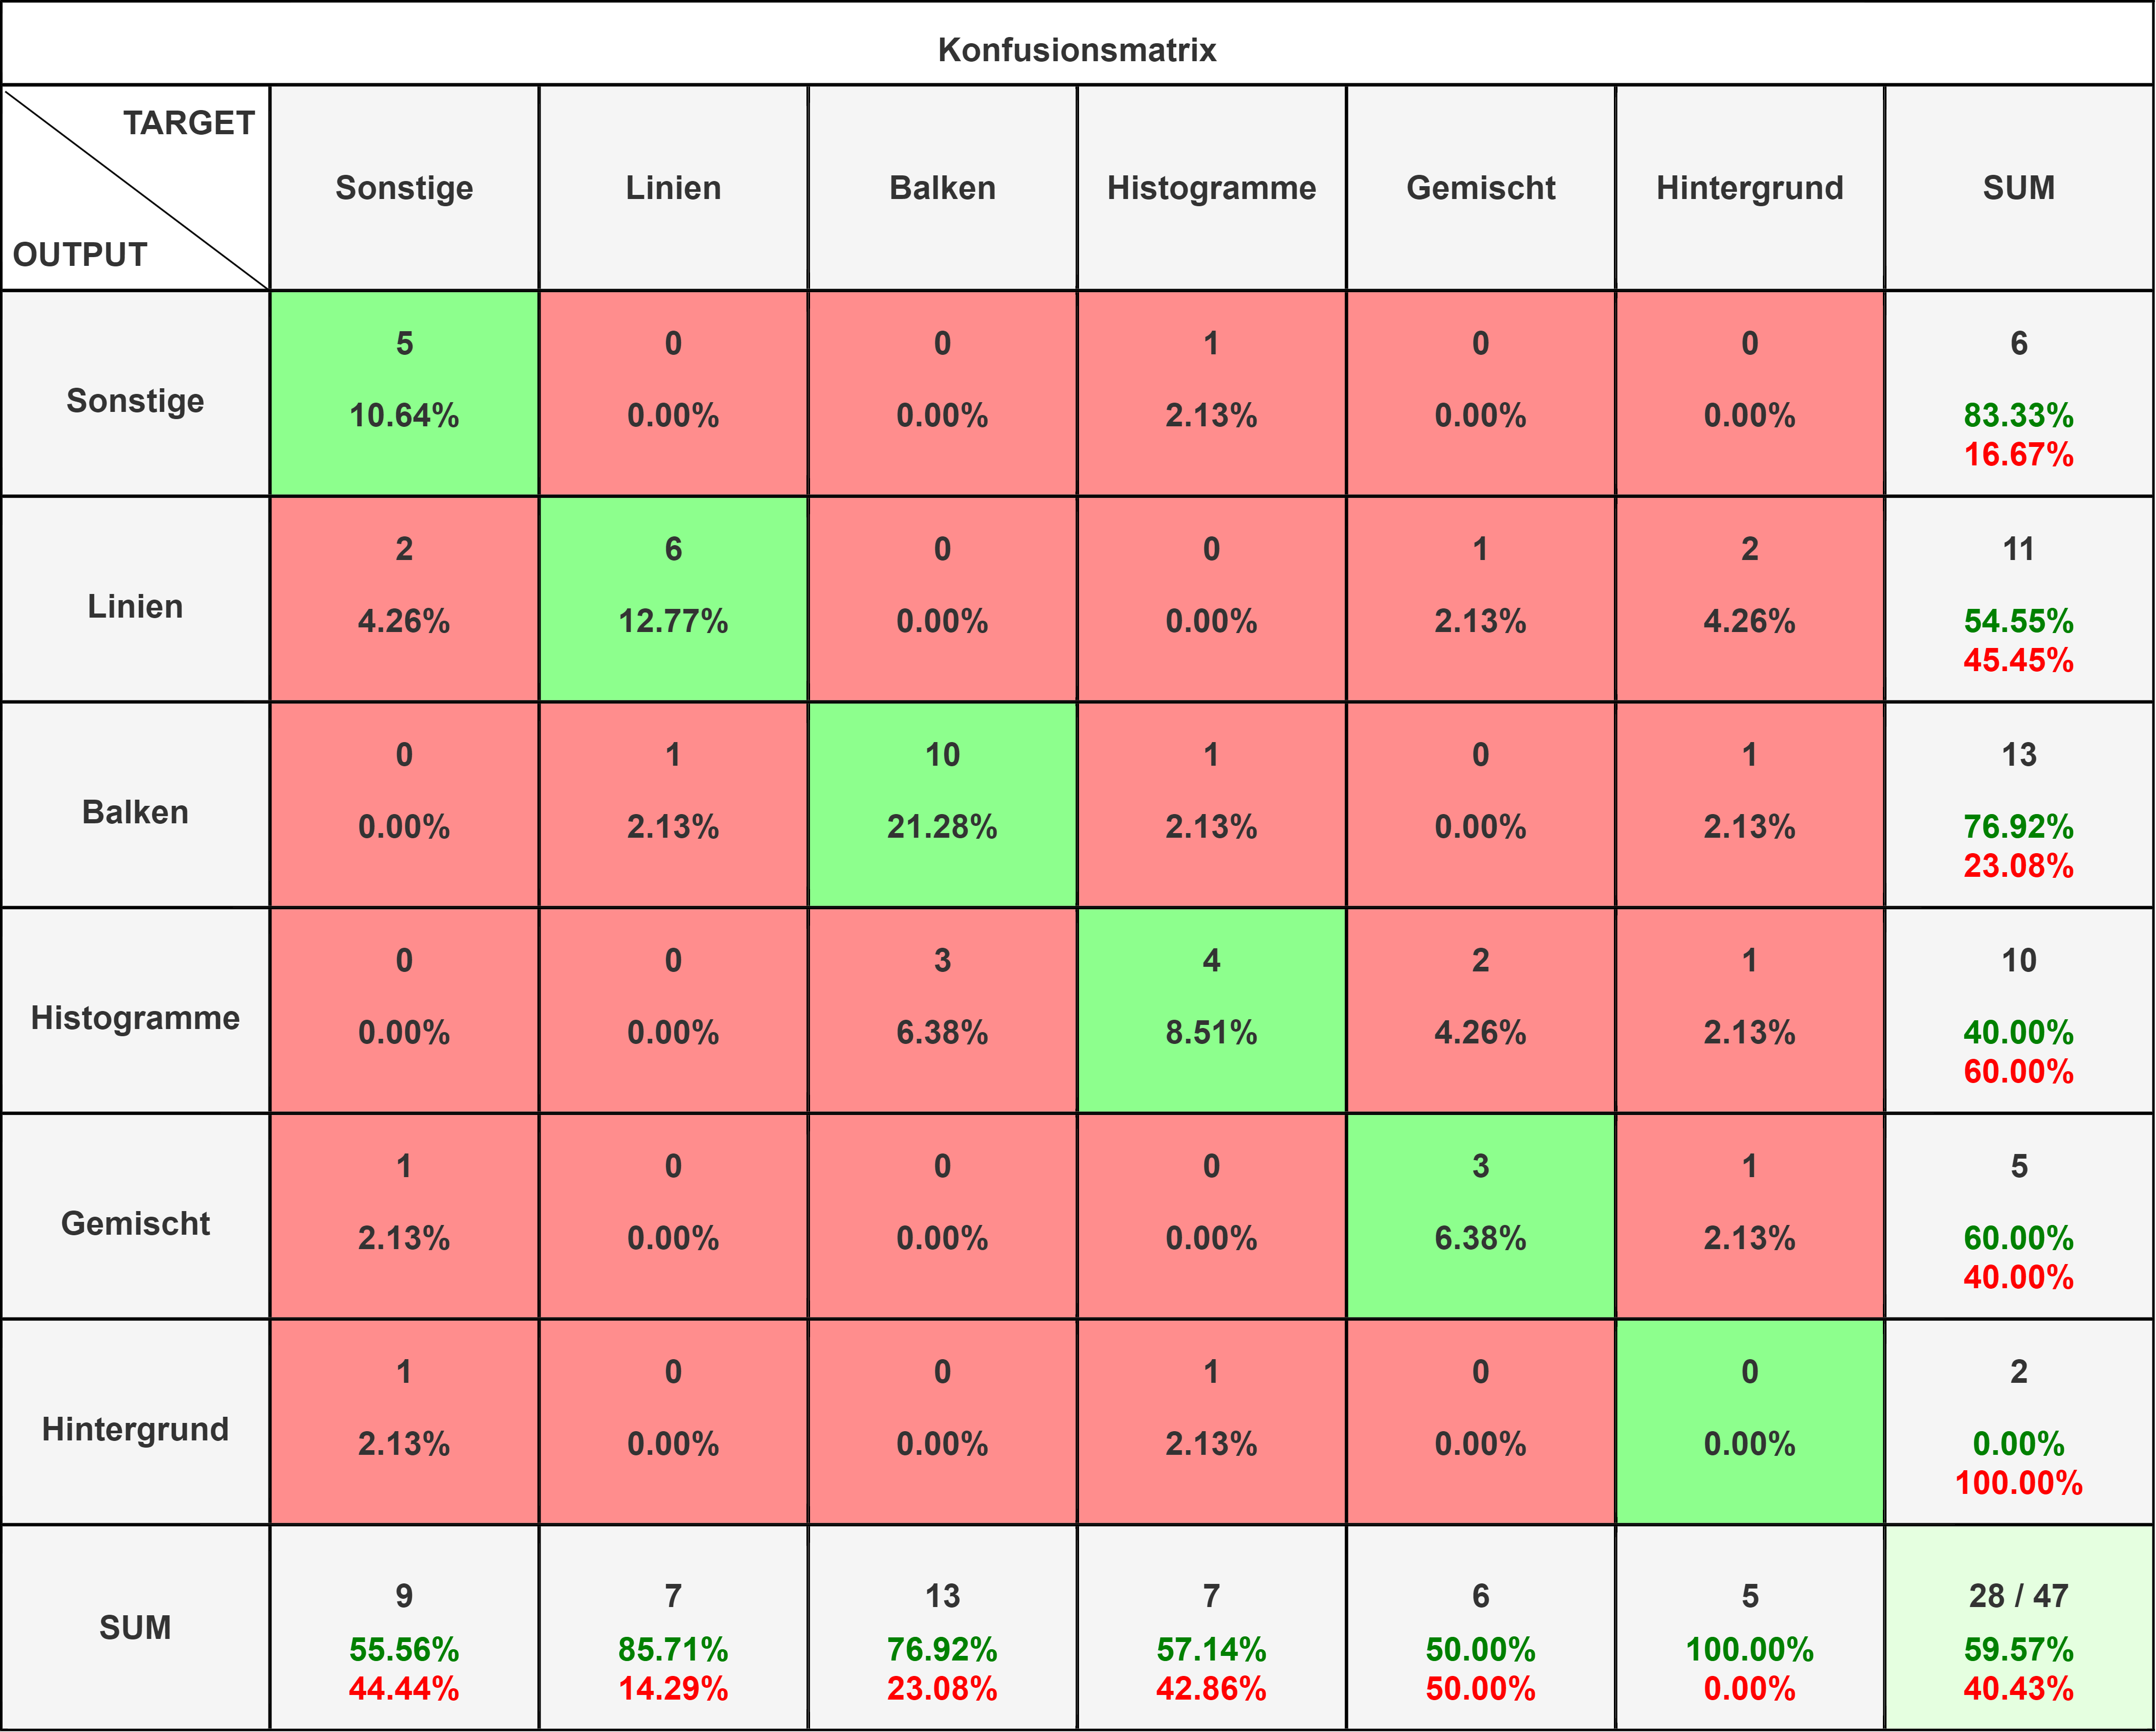
\includegraphics[width=1\textwidth]{Experimente/img/detect/1_val@0.404_200_histo/konfusionsmatrix.png}
    \caption{\hbadness=10000 x}
    \label{fig:extraction_output}
\end{figure}

\begin{table}[H]
    \centering
    \begin{tabular}{|l|c|c|c|}
        \hline
        \rowcolor[HTML]{EFEFEF}
                      & Precision        & Recall           & F1-Score         \\ \hline
        Sonstige      & 83.33\%          & 55.56\%          & 66.67\%          \\ \hline
        Linien        & 54.55\%          & 85.71\%          & 66.67\%          \\ \hline
        Balken        & 76.92\%          & 76.92\%          & 76.92\%          \\ \hline
        Histogramme   & 40.00\%          & 57.14\%          & 47.06\%          \\ \hline
        Gemischt      & 60.00\%          & 50.00\%          & 54.55\%          \\ \hline
        \textbf{Alle} & \textbf{62.96\%} & \textbf{65.07\%} & \textbf{62.37\%} \\ \hline
    \end{tabular}
    \caption{x}
\end{table}


\subsection*{200 Trainingsbilder (ohne Histogramme)}
Mit einem Konfidenzwert von 51.1\% wurden folgende Ergebnisse des Modells auf den Datensatz der reduzierten Klassenanzahl erziehlt. Auffallend sind nicht nur leichte Abweichungen der Linien und gemischten Klassen, welche der limitierten Evaluationsdatensatzgröße verschuldet sind, sondern auch deutliche Verbesserungen, der nun zusammengesetzten, Balkendiagrammsklasse.

\begin{figure}[H]
    \centering
    \captionsetup{width=1\linewidth}
    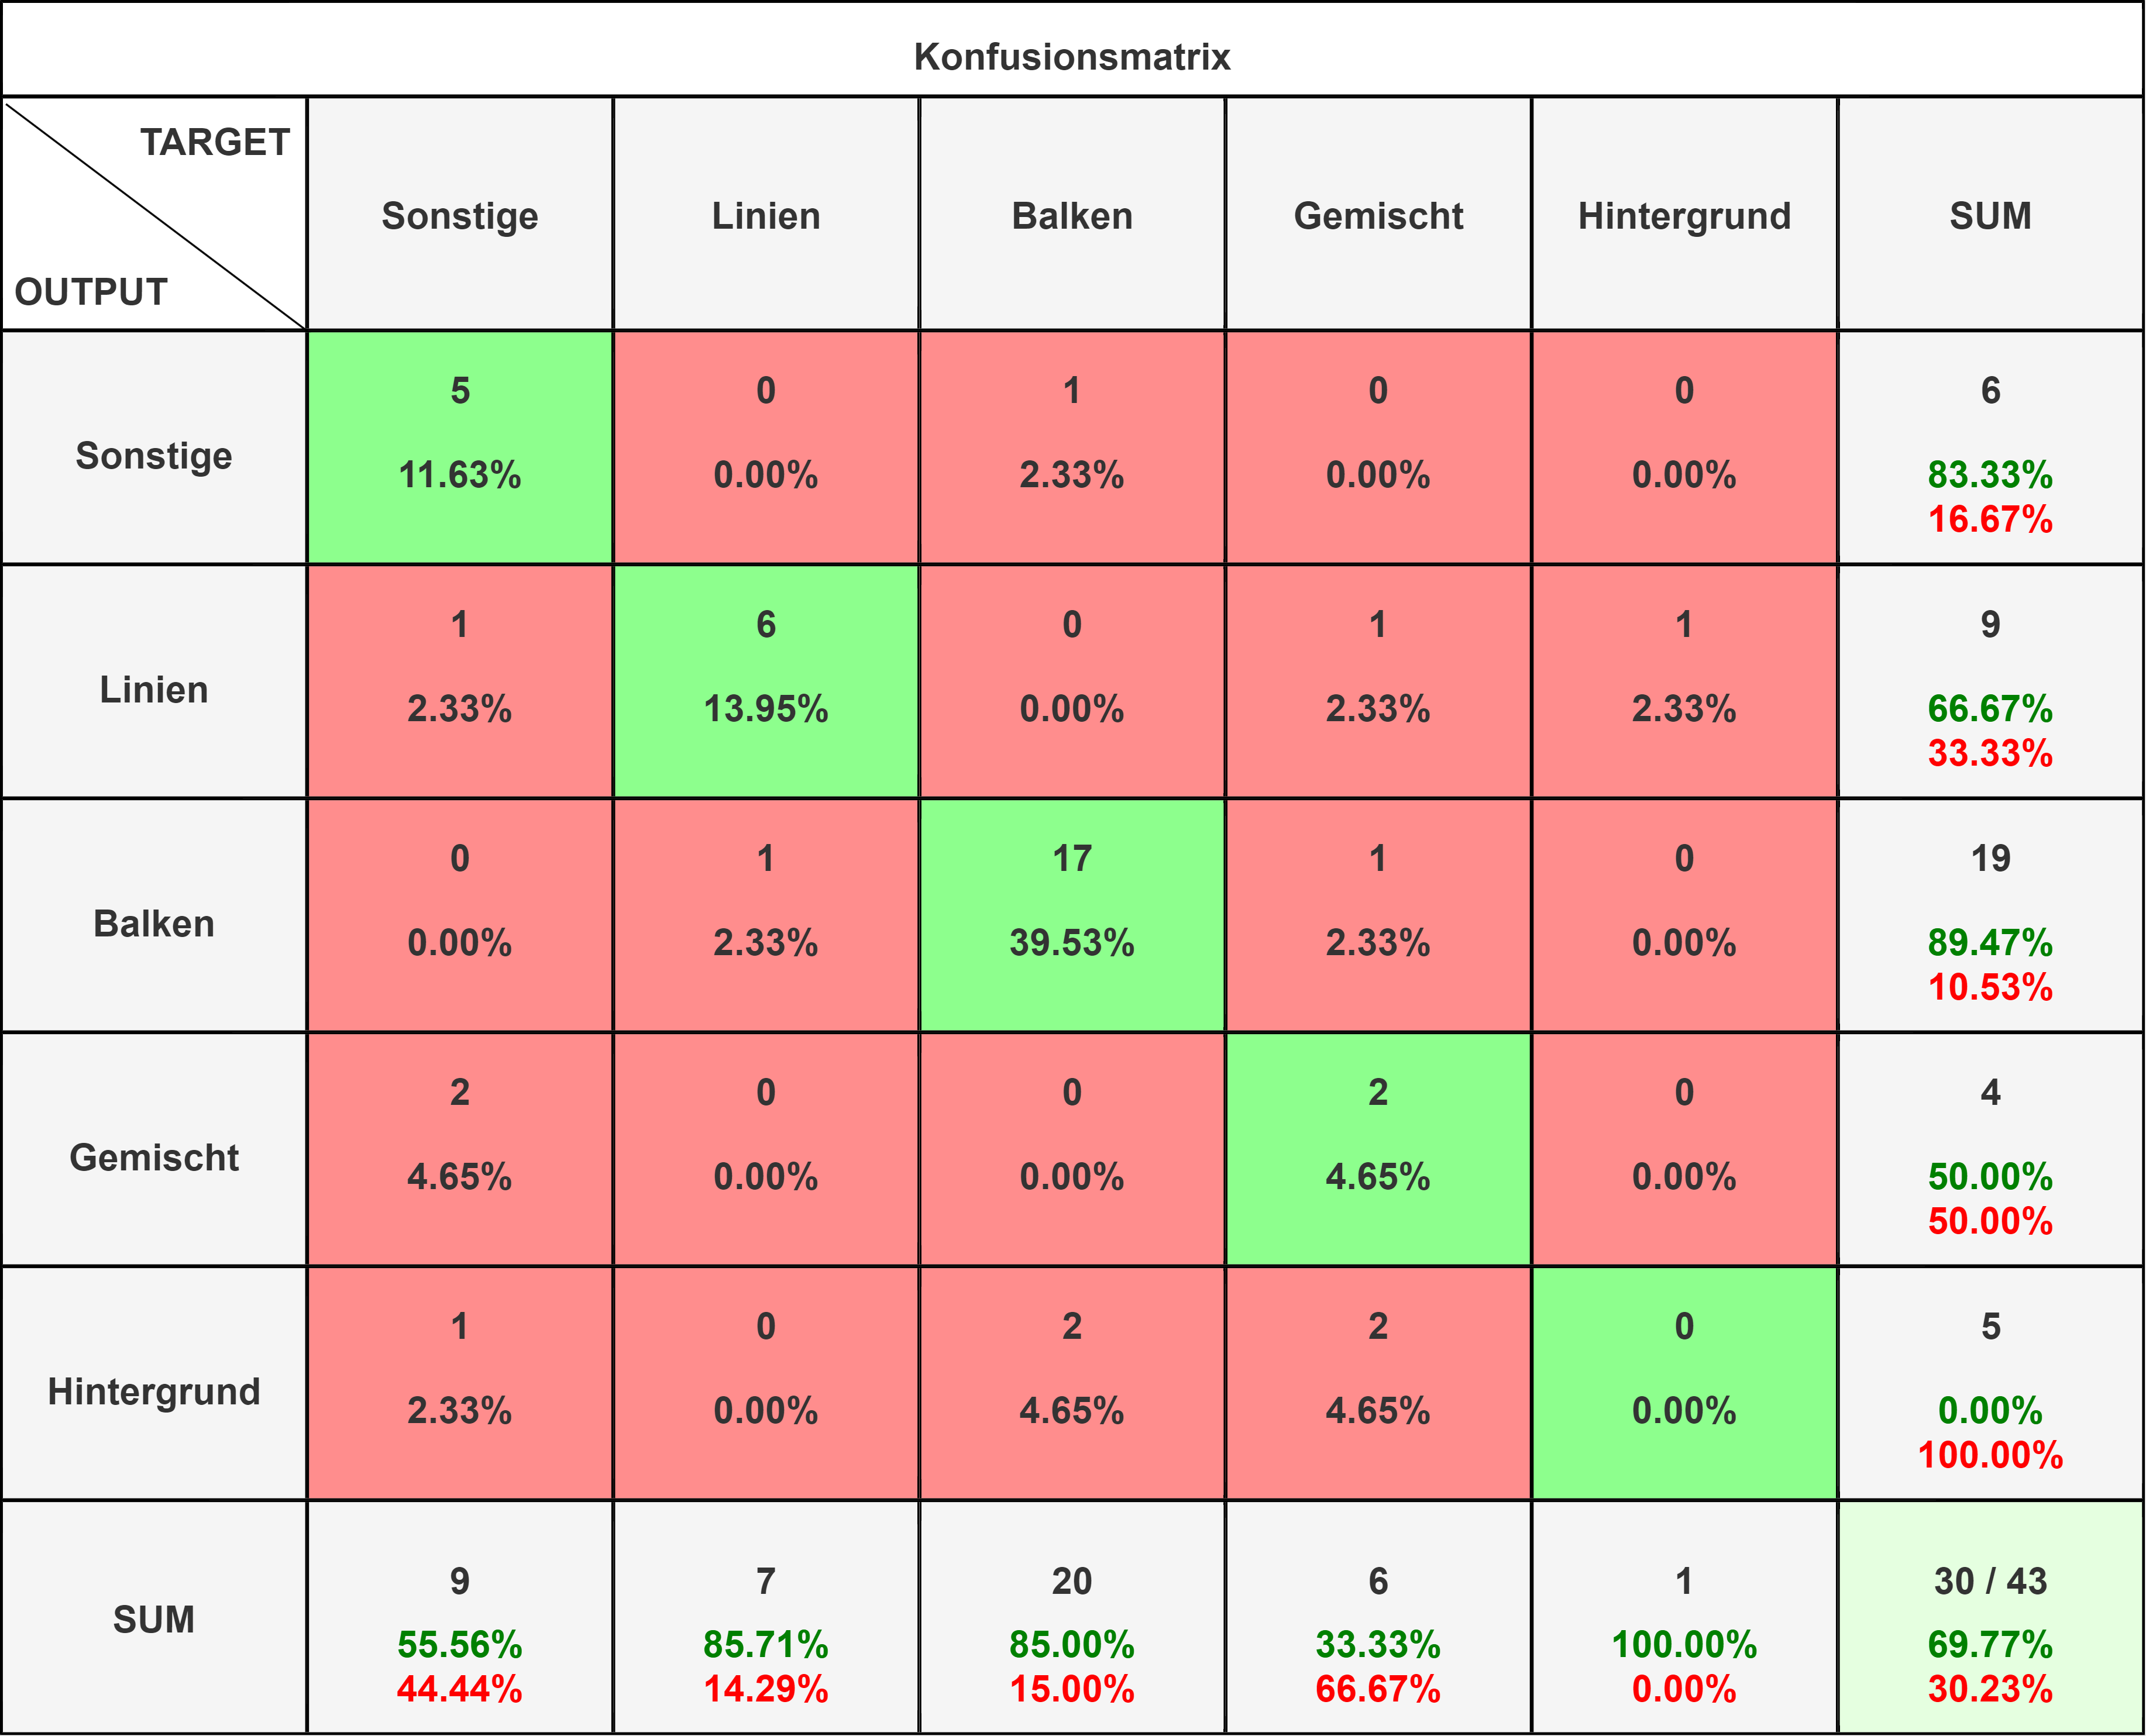
\includegraphics[width=1\textwidth]{Experimente/img/detect/2_val@0.511_200_nohisto/konfusionsmatrix.png}
    \caption{\hbadness=10000 x}
    \label{fig:extraction_output}
\end{figure}

\begin{table}[H]
    \centering
    \begin{tabular}{|l|c|c|c|}
        \hline
        \rowcolor[HTML]{EFEFEF}
                      & Precision        & Recall           & F1-Score         \\ \hline
        Sonstige      & 83.33\%          & 55.56\%          & 66.67\%          \\ \hline
        Linien        & 66.67\%          & 85.71\%          & 75.00\%          \\ \hline
        Balken        & 89.47\%          & 85.00\%          & 87.18\%          \\ \hline
        Gemischt      & 50.00\%          & 33.33\%          & 40.00\%          \\ \hline
        \textbf{Alle} & \textbf{72.37\%} & \textbf{64.90\%} & \textbf{67.21\%} \\ \hline
    \end{tabular}
    \caption{x}
\end{table}

\subsection*{321 Trainingsbilder (ohne Histogramme)}

\begin{figure}[H]
    \centering
    \captionsetup{width=1\linewidth}
    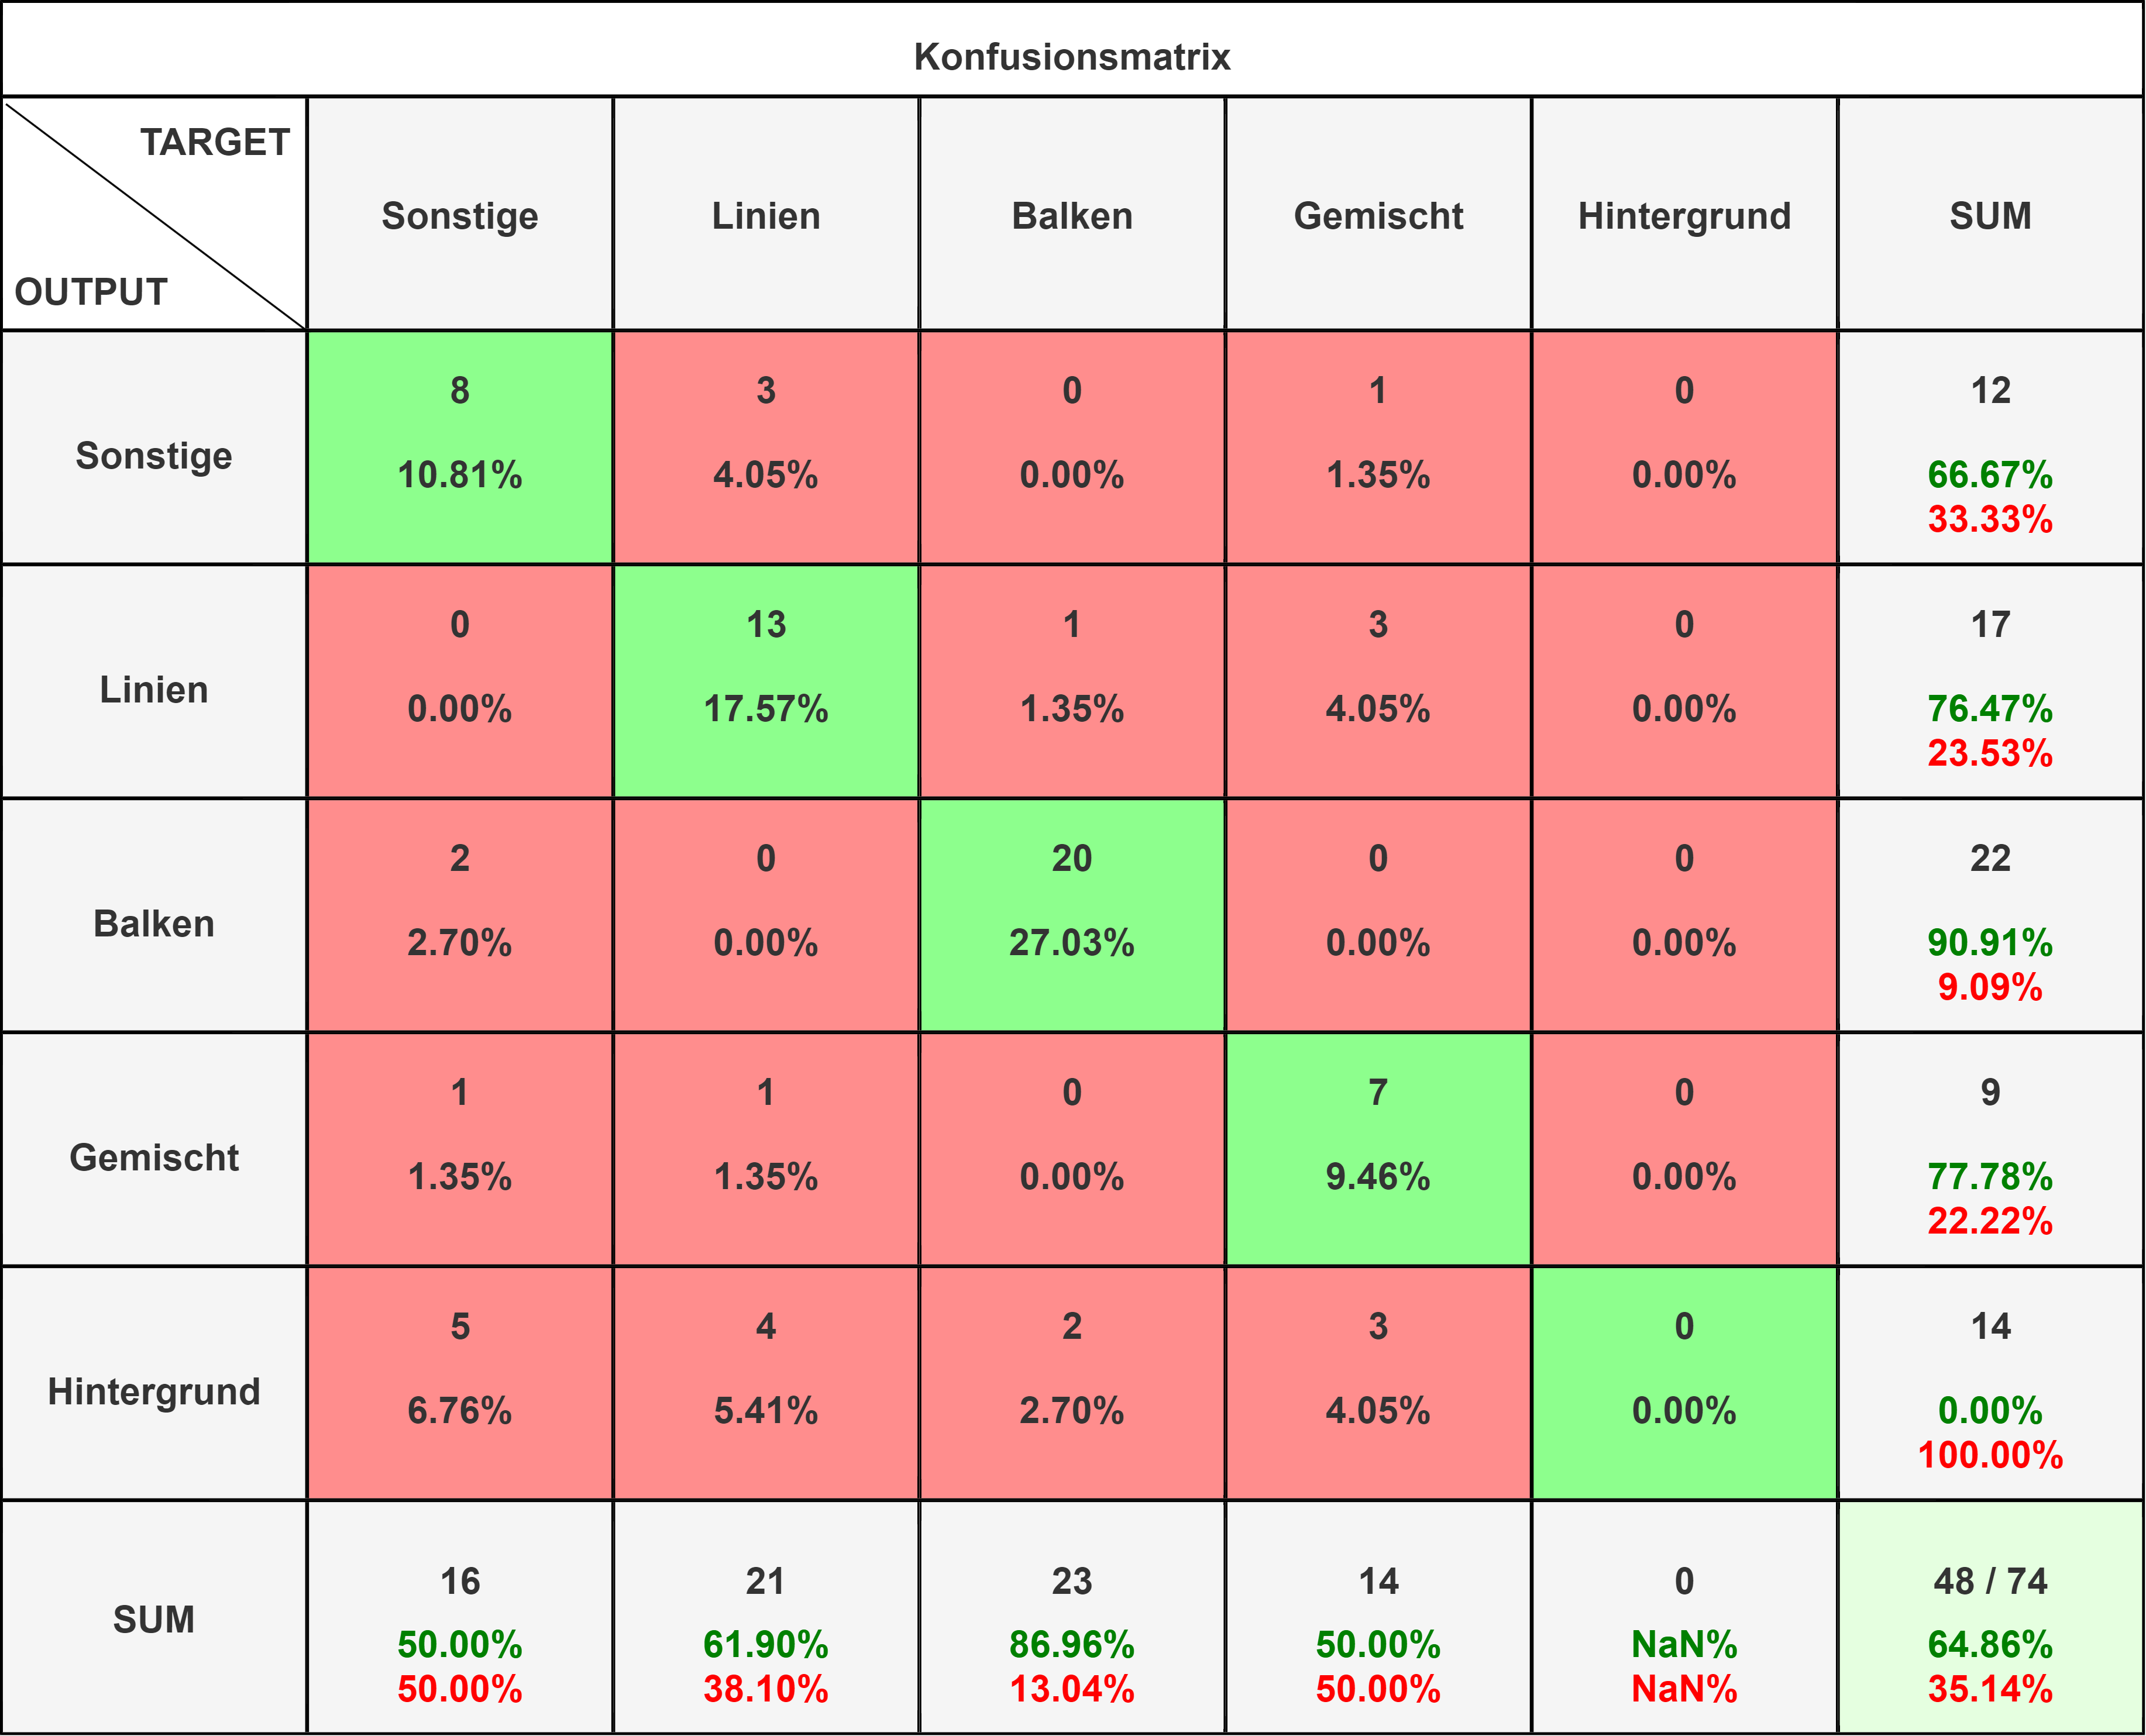
\includegraphics[width=1\textwidth]{Experimente/img/detect/3_val@0.653_nohisto/konfusionsmatrix.png}
    \caption{\hbadness=10000 x}
    \label{fig:extraction_output}
\end{figure}

\begin{table}[H]
    \centering
    \begin{tabular}{|l|c|c|c|}
        \hline
        \rowcolor[HTML]{EFEFEF}
                      & Precision        & Recall           & F1-Score         \\ \hline
        Sonstige      & 66.67\%          & 50.00\%          & 57.14\%          \\ \hline
        Linien        & 76.47\%          & 61.90\%          & 68.42\%          \\ \hline
        Balken        & 90.91\%          & 86.96\%          & 88.89\%          \\ \hline
        Gemischt      & 77.78\%          & 50.00\%          & 60.87\%          \\ \hline
        \textbf{Alle} & \textbf{77.96\%} & \textbf{62.22\%} & \textbf{68.83\%} \\ \hline
    \end{tabular}
    \caption{x}
\end{table}


\subsection{Feintraining auf historische Wirtschaftsscans}
\subsection*{2444 Trainingsbilder}
\begin{figure}[H]
    \centering
    \captionsetup{width=1\linewidth}
    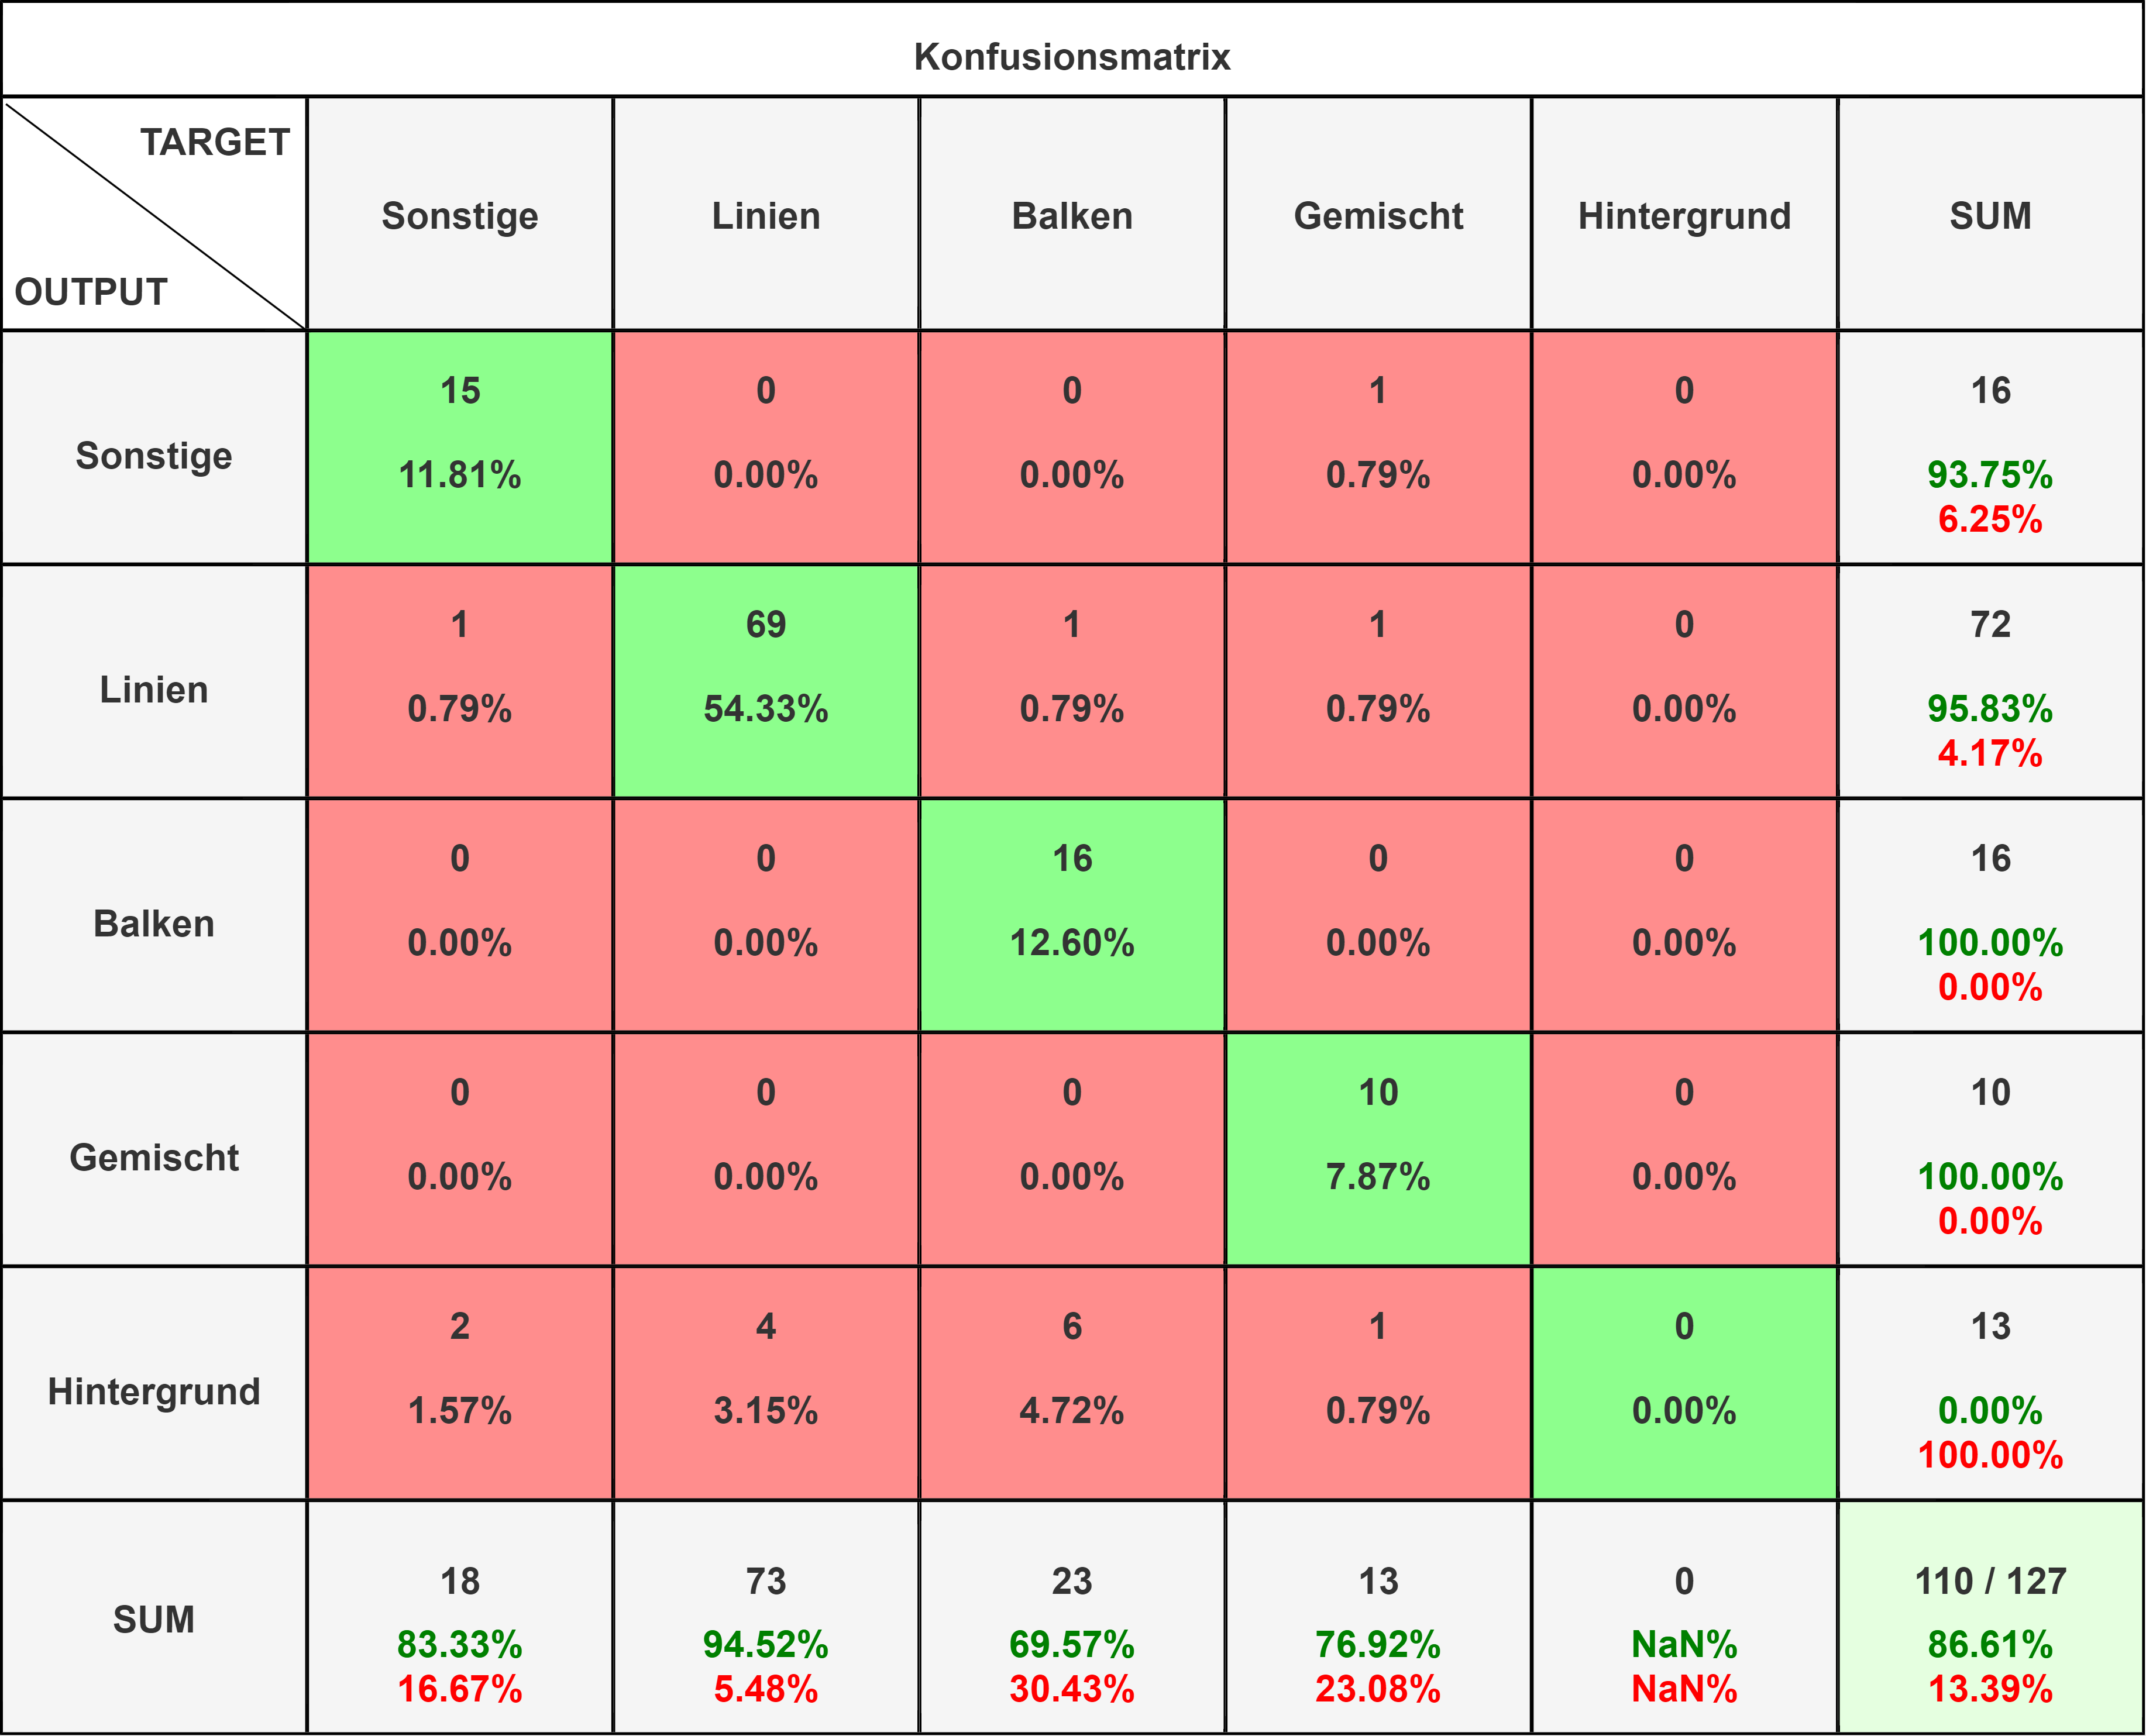
\includegraphics[width=1\textwidth]{Experimente/img/detect/val@0.891 20240612-093743_double/konfusionsmatrix.png}
    \caption{\hbadness=10000 x}
    \label{fig:extraction_output}
\end{figure}

\begin{table}[H]
    \centering
    \begin{tabular}{|l|c|c|c|}
        \hline
        \rowcolor[HTML]{EFEFEF}
                      & Precision        & Recall           & F1-Score         \\ \hline
        Sonstige      & 93.75\%          & 83.33\%          & 88.24\%          \\ \hline
        Linien        & 95.83\%          & 94.52\%          & 95.17\%          \\ \hline
        Balken        & 100.0\%          & 69.57\%          & 82.05\%          \\ \hline
        Gemischt      & 100.0\%          & 76.92\%          & 86.96\%          \\ \hline
        \textbf{Alle} & \textbf{97.40\%} & \textbf{81.09\%} & \textbf{88.11\%} \\ \hline
    \end{tabular}
    \caption{x}
\end{table}


\section{Liniendiagrammsklassifizierung}

Für die Liniendiagrammsklassifizierung wurden zwei Modelle jeweils auf die erstellten Klassifizierungsdatensätze aus \ref{ch:linebank} trainiert. Die Konfusionsmatrix \ref{fig:val_v1_matrix} macht die Schwierigkeit des Modells deutlich, überlappende und nicht überlappende Liniendiagramme zu differenzieren. Im Gegensatz zu \ref{fig:val_v2_matrix} werden hier 7 der insgesamt 19 nicht überlappenden Aufkommen falsch als überlappende Diagramme klassifiziert.

\begin{figure}[H]
    \centering
    \captionsetup{width=.75\linewidth}
    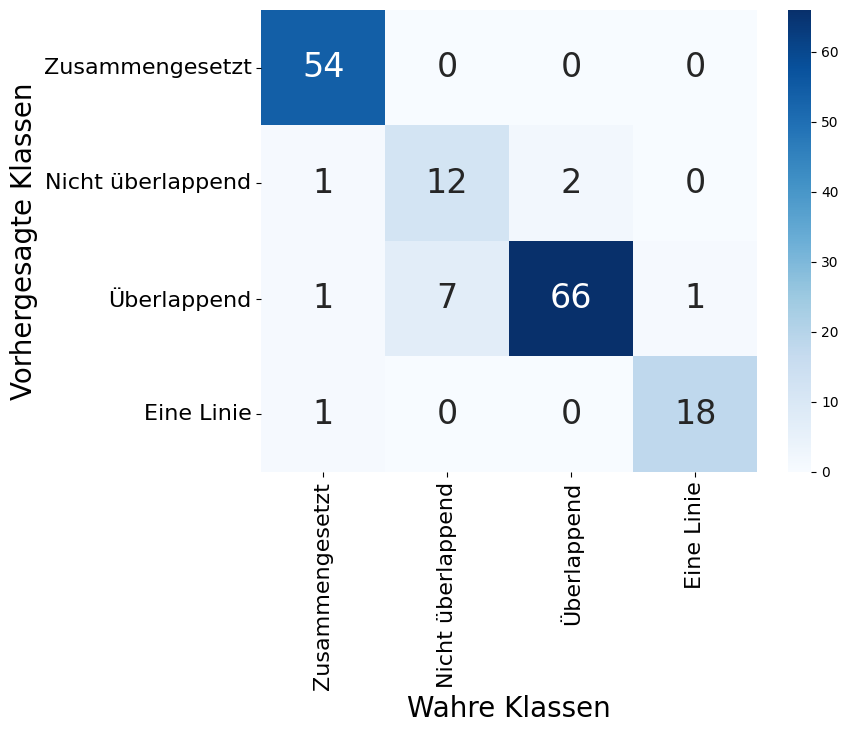
\includegraphics[width=.75\textwidth]{Experimente/img/classify/val_v1/matrix.png}
    \caption{\hbadness=10000 x}
    \label{fig:val_v1_matrix}
\end{figure}

Die besseren Ergebnisse der Unterscheidung zwischen einer und mehreren Wertelinien dagegen, spiegelt sich aber auch in der Accuracy wider: Statt 92.0\% des ersten Modells erziehlte dieses eine Klassifikationsgenauigkeit von 98.1\%.

\begin{figure}[H]
    \centering
    \captionsetup{width=.75\linewidth}
    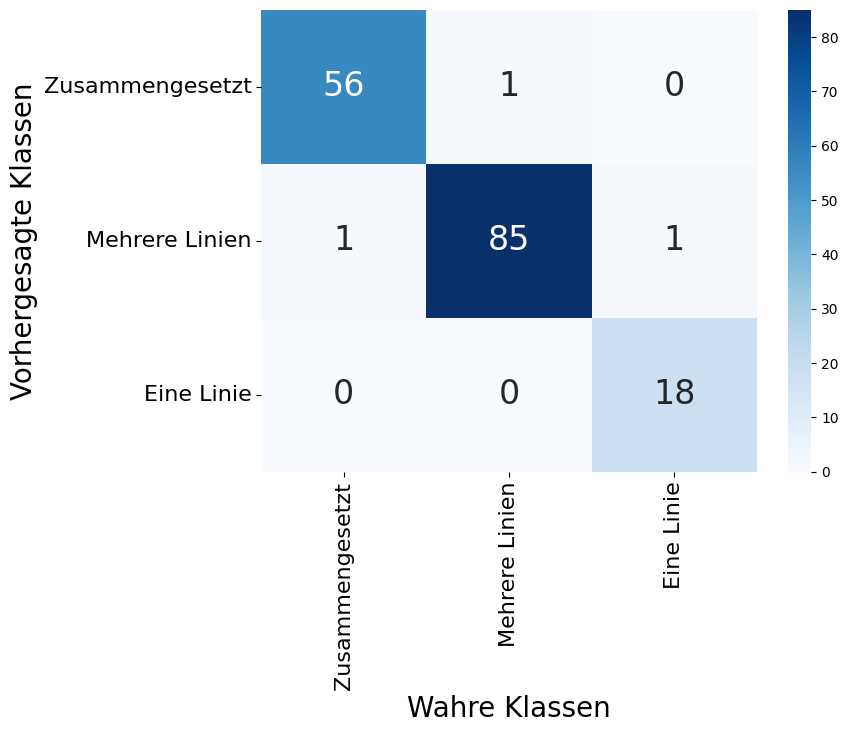
\includegraphics[width=.75\textwidth]{Experimente/img/classify/val_v2/matrix.png}
    \caption{\hbadness=10000 x}
    \label{fig:val_v2_matrix}
\end{figure}

\section{Segmentation}
\subsection{Instanzsegmentation durch Ultralytics YOLO}
\begin{table}[H]
    \centering
    \begin{tabular}{|l|c|c|c|}
        \hline
        \rowcolor[HTML]{EFEFEF}
              & Precision & Recall & F1-Score \\ \hline
        Box   & 95.6\%    & 78.8\% & 86.4\%   \\ \hline
        Maske & 93.3\%    & 76.4\% & 84.0\%   \\ \hline
    \end{tabular}
    \caption{x}
\end{table}

\subsection{Semantische Segmentation durch das U-Net}

Mit den genannten Parametern aus \ref{ch:unet} wurden insgesamt fünf verschiedene Modelle trainiert: Eines wurde auf den in \ref{ch:lines} beschriebenen Binärmaskendatensatz der Wertelinien von synthetischen Liniendiagrammen vortrainiert. Die restlichen vier Modelle wurden auf den Werteliniendatensatz der historischen Liniendiagrammen so trainiert, um jeweils den Vergleich zwischen dem Fein- und nicht Feintrainieren und der selbst eingeführten Beschreibung des \emph{32x Batch-Paddings} darzustellen. Was dieses Batch-Padding beschreibt ist lediglich die 32-fache Duplikation aller einzelnen Trainingsdatenbilder. Da jeder einzelne Bilderbatch während des Trainingsprozesses zufällig neu augmentiert wird, und so durch das Batch-Padding die limitierten Trainingsdaten möglicherweise künslich vergrößern werden könnten, wurde dies untersucht.
\\
Alle im folgenden dargestellte Ergebnisse wurden auf denselben, den der historischen Diagrammswertelinien, Validationsdatensatz evaluiert. Um die Effizienz des erstellten Datensatzgenerators anschaulich zu machen wurde das auf den synthetischen Bildern vortrainiere Modell ebenfalls auf diesem Validationsdatensatz gemessen. Allerdings wurden hier keine herausragenden Evaluationswerte erwartet, da synthetische Datensätze in der Regel nicht die Qualität von realen Daten erreichen können.

\begin{table}[H]
    \centering
    \begin{minipage}{0.475\textwidth}
        \centering
        \begin{tabular}{|l|c|c|c|}
            \hline
            \rowcolor[HTML]{EFEFEF}
                  & Precision & Recall  & F1-Score \\ \hline
            Maske & 75.55\%   & 66.19\% & 70.56\%  \\ \hline
        \end{tabular}
        \caption{Training auf synthetischem Datensatz}
    \end{minipage}%
\end{table}

Die Tauglichkeit dieser künstlichen Herangehensweise zum lediglichen Vortrainieren spiegelt sich jedoch in den unteren Tabellen wider. Besonders der Precision Wert zwischen vor- und nicht vortrainierten Modellen zeigt Verbesserungen, hier in beiden Fällen von fast 1.5\%. Recall scheint davon nicht ganz betroffen zu sein, die Verbesserungen bei dem einen und Verschlechterungen bei dem anderen können allerdings der Zufälligkeitfaktoren des Trainings verschuldet sein. Die gleichen Auffälligkeiten können im Fall des Batch-Paddings gefunden werden.

\begin{table}[H]
    \centering
    \begin{minipage}{0.475\textwidth}
        \centering
        \begin{tabular}{|l|c|c|c|}
            \hline
            \rowcolor[HTML]{EFEFEF}
                  & Precision & Recall  & F1-Score \\ \hline
            Maske & 91.52\%   & 89.36\% & 90.43\%  \\ \hline
        \end{tabular}
        \caption{Training auf vortrainiertem Modell mit 32x Batch-Padding}
    \end{minipage}%
    \hfill
    \begin{minipage}{0.475\textwidth}
        \centering
        \begin{tabular}{|l|c|c|c|}
            \hline
            \rowcolor[HTML]{EFEFEF}
                  & Precision & Recall  & F1-Score \\ \hline
            Maske & 90.41\%   & 89.57\% & 89.99\%  \\ \hline
        \end{tabular}
        \caption{Training auf vortrainiertem Modell ohne 32x Batch-Padding}
    \end{minipage}

    \vspace{1.5em} % Adjust the spacing between the rows if needed

    \begin{minipage}{0.475\textwidth}
        \centering
        \begin{tabular}{|l|c|c|c|}
            \hline
            \rowcolor[HTML]{EFEFEF}
                  & Precision & Recall  & F1-Score \\ \hline
            Maske & 89.07\%   & 89.64\% & 89.35\%  \\ \hline
        \end{tabular}
        \caption{Training auf nicht vortrainiertem Modell mit 32x Batch-Padding}
    \end{minipage}%
    \hfill
    \begin{minipage}{0.475\textwidth}
        \centering
        \begin{tabular}{|l|c|c|c|}
            \hline
            \rowcolor[HTML]{EFEFEF}
                  & Precision & Recall  & F1-Score \\ \hline
            Maske & 88.05\%   & 88.88\% & 88.46\%  \\ \hline
        \end{tabular}
        \caption{Training auf nicht vortrainiertem Modell ohne 32x Batch-Padding}
    \end{minipage}
\end{table}


% \begin{table}[H]
%     \centering
%     \begin{tabular}{|l|c|c|c|}
%         \hline
%         \rowcolor[HTML]{EFEFEF}
%               & Precision & Recall  & F1-Score \\ \hline
%         Maske & 91.52\%   & 89.36\% & 90.43\%  \\ \hline
%     \end{tabular}
%     \caption{Training auf vortrainierten Modell mit 32x Batch-Padding}
% \end{table}

% \begin{table}[H]
%     \centering
%     \begin{tabular}{|l|c|c|c|}
%         \hline
%         \rowcolor[HTML]{EFEFEF}
%               & Precision & Recall  & F1-Score \\ \hline
%         Maske & 90.41\%   & 89.57\% & 89.99\%  \\ \hline
%     \end{tabular}
%     \caption{Training auf vortrainierten Modell ohne 32x Batch-Padding}
% \end{table}

% \begin{table}[H]
%     \centering
%     \begin{tabular}{|l|c|c|c|}
%         \hline
%         \rowcolor[HTML]{EFEFEF}
%               & Precision & Recall  & F1-Score \\ \hline
%         Maske & 89.07\%   & 89.64\% & 89.35\%  \\ \hline
%     \end{tabular}
%     \caption{Training auf nicht vortrainierten Modell mit 32x Batch-Padding}
% \end{table}

% \begin{table}[H]
%     \centering
%     \begin{tabular}{|l|c|c|c|}
%         \hline
%         \rowcolor[HTML]{EFEFEF}
%               & Precision & Recall  & F1-Score \\ \hline
%         Maske & 88.05\%   & 88.88\% & 88.46\%  \\ \hline
%     \end{tabular}
%     \caption{Training auf nicht vortrainierten Modell ohne 32x Batch-Padding}
% \end{table}

\section{Diagrammsauswertung}
\subsection{Achsenerkennung durch OCR}
\begin{table}[H]
    \centering
    \begin{tabular}{|c|c|c|c|}
        \hline
        \rowcolor[HTML]{EFEFEF}
        Titel & Linke Y-Achse & Rechte Y-Achse & X-Achse \\ \hline
        3     & 0             & 1              & 10      \\ \hline
    \end{tabular}
    \caption{Von den 27 Fehlern wegen fehlerhaftem Achsenerkennungsalgorithmus}
\end{table}

\begin{table}[H]
    \centering
    \begin{tabular}{|c|c|c|c|}
        \hline
        \rowcolor[HTML]{EFEFEF}
        Titel & Linke Y-Achse & Rechte Y-Achse & X-Achse \\ \hline
        6     & 6             & 4              & 10      \\ \hline
    \end{tabular}
    \caption{Von den 27 Fehlern wegen fehlerhafter optischen Schriftzeichenerkennung}
\end{table}




\subsection{Numerische Tabellenformextraktion}



Im Kapitel "Experimente" Ihrer Bachelorarbeit sollten Sie die durchgeführten Versuche, deren Ergebnisse und Ihre Analyse darlegen. Hier ist eine Übersicht der wichtigsten Punkte, die in diesem Kapitel enthalten sein sollten:

Versuchsaufbau:

Beschreibung der verwendeten Datensätze (Trainings-, Validierungs- und Testdaten)
Erklärung der Evaluierungsmetriken (z.B. mAP für YOLO, IoU für U-Net)
Definition der Baseline oder Vergleichsmodelle


Durchgeführte Experimente:

Detaillierte Beschreibung jedes einzelnen Experiments
Begründung für die Wahl der Experimente
Variationen in Hyperparametern, Modellarchitekturen oder Trainingsmethoden


Ergebnisse:

Präsentation der quantitativen Ergebnisse (in Tabellen oder Grafiken)
Qualitative Ergebnisse (z.B. Beispielbilder von Vorhersagen)
Vergleich der Leistung von YOLO und U-Net für Ihre spezifische Aufgabe


Analyse:

Interpretation der Ergebnisse
Diskussion von Stärken und Schwächen der Modelle
Vergleich mit dem aktuellen Stand der Technik oder anderen relevanten Arbeiten


Ablationstudie:

Untersuchung des Einflusses verschiedener Komponenten oder Hyperparameter auf die Modellleistung


Fehleranalyse:

Identifikation von häufigen Fehlertypen
Diskussion möglicher Gründe für diese Fehler


Laufzeitanalyse und Ressourcenverbrauch:

Vergleich der Inferenzzeiten von YOLO und U-Net
Analyse des Speicher- und Rechenbedarfs


Diskussion der Limitationen:

Grenzen der durchgeführten Experimente
Mögliche Verzerrungen in den Daten oder der Evaluation


Zukünftige Arbeiten:

Vorschläge für weitere Experimente oder Verbesserungen basierend auf Ihren Ergebnissen



Dieses Kapitel sollte eine objektive Darstellung Ihrer experimentellen Arbeit sein, die es dem Leser ermöglicht, die Leistung und Eignung von YOLO und U-Net für Ihre spezifische Anwendung zu verstehen und zu bewerten.